% UG project example file, February 2024
%
%   Added the "online" option for equal margins, February 2024 [Hiroshi Shimodaira, Iain Murray]
%   A minor change in citation, September 2023 [Hiroshi Shimodaira]
%
% Do not change the first two lines of code, except you may delete "logo," if causing problems.
% Understand any problems and seek approval before assuming it's ok to remove ugcheck.
\documentclass[logo,bsc,singlespacing,parskip,online]{infthesis}
\usepackage{ugcheck}


% Include any packages you need below, but don't include any that change the page
% layout or style of the dissertation. By including the ugcheck package above,
% you should catch most accidental changes of page layout though.

\usepackage{microtype} % recommended, but you can remove if it causes problems
\usepackage[square,numbers]{natbib} % recommended for citations
\usepackage{graphicx}
\usepackage{amssymb}
\usepackage{amsmath}
\graphicspath{ {./images/}}
\usepackage{natbib}
\bibliographystyle{abbrvnat}
\setcitestyle{authoryear,open={(},close={)}} %Citation-related commands

\begin{document}
\begin{preliminary}

% \title{Investigating Machine Learning Techniques for Hearing Aids}
\title{Towards a State-Dependent Model for Speech Enhancement in Hearing Aids}

\author{Nikodem Bieniek}

%\course{Artificial Intelligence and Computer Science}
\course{Master of Informatics} % MInf students

\project{MInf Project (Part 1) Report}  % 4th year MInf students
%\project{MInf Project (Part 2) Report}  % 5th year MInf students


\date{\today}

\abstract{
   This dissertation explores the intersection of Machine Learning, Automatic Speech Recognition (ASR) and Hearing Aids (HA) 
   through the lens of Acoustic Scene Analysis (ASA) and Speech Enhancement (SE).
   The primary objective of this dissertation is to develop machine learning models capable of prioritising 
   speech in noisy environments whilst remaining computationally feasible for implementation in hearing aids.
   The vision is to chain the ASA and SE models together to form a state-dependent model, 
   which leverages a-priori knowledge of the acoustic scene to suitably enhance the speech in the environment.

   While there is a growing trend in academia to use deep neural networks (DNNs) for ASA and SE, 
   they often overlook the computational constraints of the devices 
   and even more so for HAs. Consequently, each proposed model is evaluated not only in terms of performance but also on its feasibility for real-time deployment, as measured by metrics such as Floating Point Operations Per Second (FLOPS) and the number of model parameters.
   
   Additionally, there is a growing trend in the market to incorporate deep neural networks (DNNs) into hearing aids.
   This could be due to the increasing computational capabilities of the devices, 
   and the potential for it to improve the quality of life for hearing aid users 
   over non-neural network based approaches.
   Evidence from state of the art manufacturers suggests that a combination of ASA and SE techniques are employed,
   further motivating the approach adopted in this project. 
   There is also more insight into the computational capabilities of the devices, 
   which allows for more up-to-date feasibility comparisons.
   
   Experiments are conducted primarily on a novel dataset called HEAR-DS -
   one of the few datasets that is specifically designed for HA research.
   As a baseline, the Convolutional Neural Network (CNN) ASA model presented by the authors of the dataset is utilised.
   We will demonstrate improvements in both the training procedure and the generalisation capability 
   of the baseline CNN through the implementation of data augmentation strategies and the adoption of an alternative optimiser.
   
   Furthermore, the dataset is extended by demonstrating a proof-of-concept of a speech enhancement model 
   using a shallow CNN model that works in the frequency-time domain. We evaluate the performance of the model 
   using artificial intelligibility and quality metrics such as STOI and PESQ. While the performance is not on par 
   with the state-of-the-art, it most certainly motivates further research in the next part of the dissertation.
}

\maketitle

\newenvironment{ethics}
   {\begin{frontenv}{Research Ethics Approval}{\LARGE}}
   {\end{frontenv}\newpage}

\begin{ethics}
This project was planned in accordance with the Informatics Research
Ethics policy. It did not involve any aspects that required approval
from the Informatics Research Ethics committee.

\standarddeclaration
\end{ethics}


\begin{acknowledgements}
First and foremost, I would like to solemly thank my supervisor, Hao Tang for 
his enthusiasm in guiding me through this self-proposed dissertation. I am eternally grateful for his wisdom, guidance, and patience throughout the project.

I would like to also thank my friends, for their support and encouragement throughout the project. 

And to my parents, without whose sacrifices I would not have been able to pursue this degree, let alone this project.
\end{acknowledgements}


\tableofcontents
\end{preliminary}


\chapter{Introduction}
\section{Motivations}
Hearing loss is a prevalent condition affecting as much as 
430 million people - or 1 in 18 people. This is expected 
to rise to 1 in 10 by 2050 \citep{WHO2024deafness}.
The most common treatment for hearing loss is the 
provision of hearing technology - such as Hearing Aids (HAs) or cochlear implants.
There are many types of HAs, but the most common
type is the behind-the-ear (BTE) hearing aid \citep{Kochkin2010MarkeTrak8}.
However, HA users often report that they struggle to hear speech
in noisy environments. For example, in the study by \citet{Kochkin2010MarkeTrak8},
42\% of HA users reported that wind noise was a significant issue for them.
This project aims to evaluate the effectiveness of machine learning algorithms
in prioritising the speech in various environments (such as windy environments).

Modern hearing aids now apply a wide range of techniques to achieve 
better speech prioritisation. For wind noise reduction, this can be achieved 
from mechanical solutions - product design to covers that reduce wind noise - to 
signal processing techniques to compensate for mechanical limitations.
However, current techniques are still not perfect as shown by the study from \citet{Kochkin2010MarkeTrak8}.

Wind noise reduction and indeed, noise reduction in general, is a challenging problem
when paired with speech. This is because you have 
to strike a balance between reducing background noise and
preserving speech. 
\citet{Korhonen2021WindNoise} outlines 
various techniques that could be used to reduce the wind noise in hearing aids -
from modulation-based noise reduction algorithms (Wiener filtering),
adaptive filtering algorithms, to machine learning techniques.
The paper mentions that the the proposed ML technique:
Long Short-Term Memory (LSTM) neural networks provided
modest improvements in wind noise reduction, however, it did highlight
that ML techniques may still have utility through further research 
and careful algorithmic choices. 

This project aims to investigate the effectiveness of machine learning techniques 
in prioritising speech in noisy environments. The idea is to 
first train a deep neural network (DNN) to perform acoustic scene analysis (ASA) to classify the environment.
Afterwards, a speech enhancement model will be trained to enhance the speech in the environment.
From now on, we will refer to the chaining of the ASA and SE models together as a state-dependent model
as inspired by \citet{katagiri_handbook_2000}'s categorisation of SE techniques (see \ref{sec:background:se} for more details).

In this project, we will be using a novel dataset proposed by \citet{Huwel2020HearDS}.
This dataset (called HEAR-DS) is unique because it is specially tailored for HA signal processing and contains
various environments. Normally, voice activity detection (VAD) would be 
used to detect speech, however, we will take inspiration from \citet{Huwel2020HearDS}
by mixing the samples with speech and label them as so. 
This can be used to implicitly train the machine learning model to classify the environment 
and whether speech is present.
%  Additionally, the paper presents an 
% elementary example of how the dataset can be used: to classify the environment -
The paper also presents an example of a task that can be performed on the dataset, 
namely, ASA. It showcases the use of a convolutional neural network (CNN) to classify the environment.
This dissertation will be extending the paper by looking at how HEAR-DS can be used 
to additionally train a speech enhancement model 
and to ultimately chain the ASA and SE models together to form a state-dependent model.

The project will also be mindful in its algorithmic choices - as the computational
power required in HA is limited. It is difficult to pinpoint the exact computational power of a HA
due to the proprietary nature of the devices. In August 2024,
Phonak (Sonova Holding AG) released a new HA which is their first AI 
equipped HA. The device is said to be capable of handling 7,700 Million 
Operations Per Second to accommmodate its neural network with 4.5 million parameters \citep{Hasemann2024PhonakSphere}.  Contrast this with a paper 
from 2021 investigating techniques in VAD for hearing aids 
quotes that it `rarely exceeds 5 million instructions per second` \citep{Gomez2021MIPS}.
Moreover, Apple's release of a FDA approved hearing aid in which was previously a mainstream earphone wearable,
Apple Airpods, also shows that there's more interest in this area \citep{Apple2025Airpods}.
So suffice to say, the computational power of hearing aids is accelerating 
and is most likely going to continue to grow given the increasing demand 
for HAs.

Delay constraints also play a critical role in HA performance, as real-time speech perception is essential for user satisfaction.
Prior research suggests that a delay of up to 30 milliseconds (ms), and ideally less than 20ms, the user
is unaffected by the delay \citep{Stone2002Delays}. Therefore, the project will be mindful in its algorithmic choices to ensure that the model
is computationally efficient and feasible for real-time deployment.

The main evaluation metrics we will consider in this part of the dissertation 
is short-time objective intelligibility (STOI) and perceptual evaluation of speech quality (PESQ). 
These are both artificial metrics and give an indication of the quality of the speech enhancement model. 
Their limitations are discussed in chapter \ref{chap:discussion}, with subsequent sections outlining strategies to address these shortcomings.
Additionally, informed by current state-of-the-art HA configurations, the project will also assess model complexity by analysing the number of weights utilised in our designs.

The project is predominantly aimed at the hearing aid industry. If successful, the project
could advance the state-of-the-art techniques in hearing aids which 
could improve the quality of life for hearing aid users.
There is also potential to extend the work to other fields that deal with audio signal processing,
such as mainstream wearables like headphones or microphones.
% A secondary goal is to make hearing aid research more accessible to the 
% computer science community.


\section{Structure}
Going forward, the dissertation will be structured as follows:
\begin{itemize}  
   \item \textbf{Chapter \ref{ch:background}} - This chapter will give a high level overview of hearing loss, the auditory system, and the speech processing concepts needed to understand the project.
   We briefly also cover the two techniques that will be used in this project: Acoustic Scene Analysis (ASA) and Speech Enhancement
   and some of the related work done in the field. Lastly, I mention the criticism of the paper by \citet{Huwel2020HearDS} 
   that I will be exploring in this project.
   \item \textbf{Chapter \ref{ch:methodology}} - lorem ipsum
   TODO
   % \item \label{ch:Methodology} - This chapter will give a high level overview of the 
   % methodology used in this project. It will cover the datasets that will be used, the baseline models that will be used, and the hypotheses that will be tested.
   % \item \label{ch:Results} - This chapter will cover the results of the experiments.
   % \item \label{ch:Discussion} - This chapter will discuss the results of the experiments and the implications of the results.
   % \item \textbf{Experimental Setup} - This chapter will cover the datasets that will be used in this project, the baseline models that will be used, and the hypotheses that will be tested.
   % \item We then move onto the results of the experiments.
   % \begin{itemize}
   %    \item \textbf{Acoustic Scene Classification} - This section will cover the results of the experiments pertaining to the ASA task.
   %    \item \textbf{Speech Enhancement} - This section will cover the results of the experiments pertaining to the speech enhancement task.
   % \end{itemize}
   % \item \textbf{Discussion/Conclusion} - This chapter will discuss the results of the experiments and the implications of the results.
\end{itemize}
 

\chapter{Background}
\label{ch:background}

\section{Hearing Loss}
To fully appreciate the topic of this dissertation,
we will give a high level overview of the auditory system 
which is ultimately responsible for our ability to hear.
We will then cover how hearing loss can occur, and 
what solutions have been developed to help those with hearing loss.
\subsection{Auditory System}
For sound to be registered by humans, it has to travel through the ear to transform them into
what is known as a neural impulse which is then trasmitted to the brain. We will 
give a high level overview of how this process occurs which was collated by the phonetics textbook from \citet{Wayland2018Phonetics},
 but for further reading, refer to the textbook. 

 This process of sound to be registered by humans, is all done in what's known as the Auditory System.
 Figure \ref{fig:ear} shows a birds eye view of the auditory system, and it can be split into three segments
 that we will explore below.

\begin{figure}[h]
   \centering
   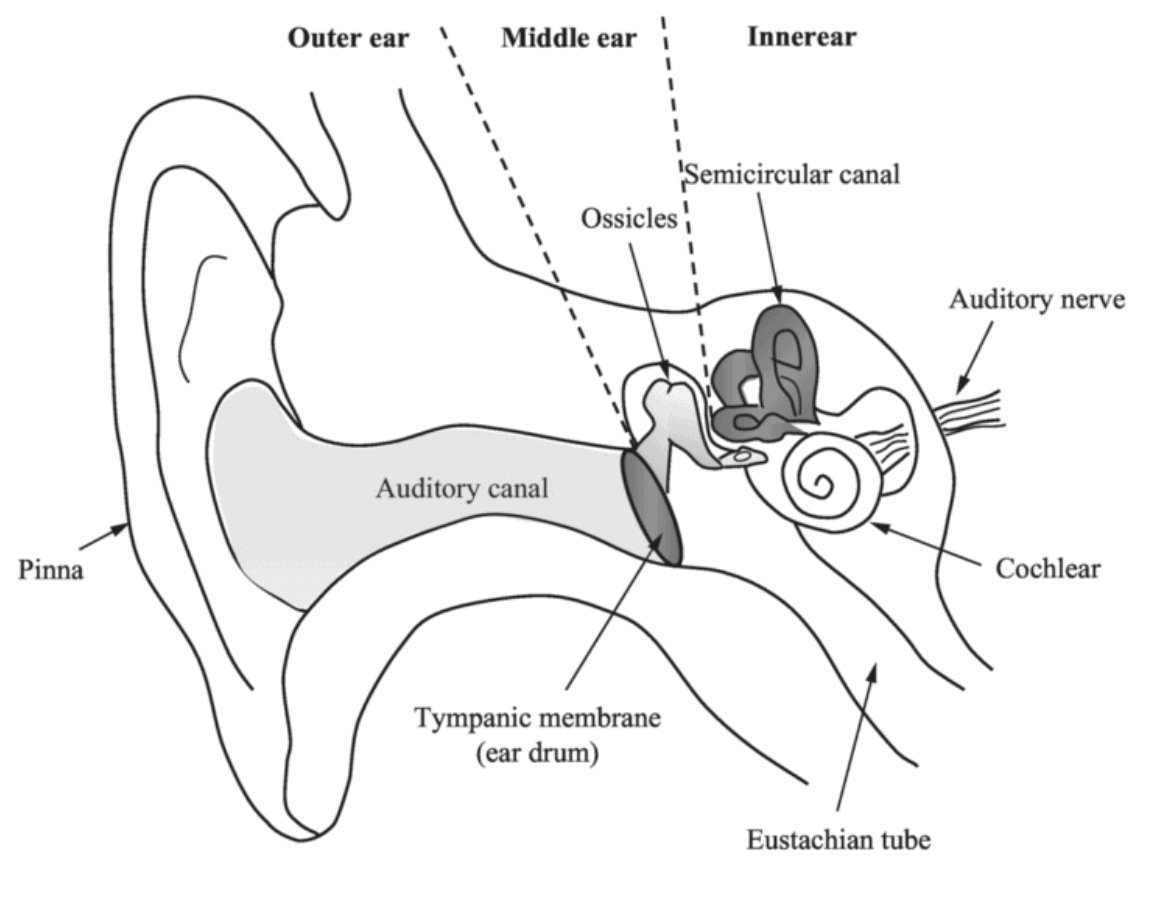
\includegraphics[width=0.5\textwidth]{wayland-ear}
   \caption{The external, middle and the inner ear from \citet{Wayland2018Phonetics}}
   \label{fig:ear}
\end{figure}

\subsubsection{The Outer Ear}
The outer ear (sometimes referred to as the External Ear) is responsible for channeling sound waves to the tympanic membrane (ear drum). Firstly,
sound waves reach the Pinna (the part of the ear that we can see and touch) which funnels it through the auditory canal, and at the end of the canal 
is the ear drum, at which point the sound waves collide with the ear drum which causes the ear drum to vibrate. 
The vibrations are passed along to the middle ear.

\subsubsection{The Middle Ear}
Zooming into the middle ear (Figure \ref{fig:middle-ear}), there are three bony structures: the Malleus, Incus, and Stapes,
and together they make up a lever system. 
It is worth pointing out that when transmitting the energy from the ear drum to the middle ear, there is bound to be some energy 
loss which can be as high as 40\%. The lever system's mechanical advantage 
allows for the sound energy to be amplified so the loss of energy is compensated. 

The Stapes also has an additional function besides passing over the sound vibrations to the inner ear. The Stapes 
is connected by a muscle, the Stapedius muscle, and in response to loud noises, it temporarily increases the stifness
of the bones in the middle ear, which temporarily prevents the acoustic energy to be amplified. This 
protects the inner ear from loud noises.

\begin{figure}[h]
   \centering
   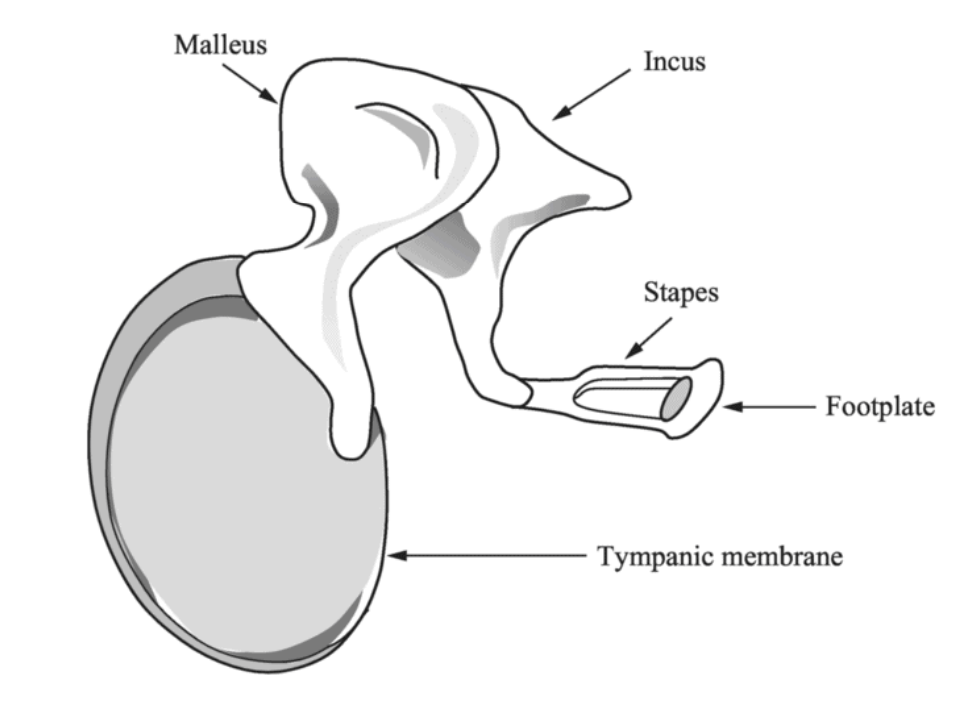
\includegraphics[width=0.5\textwidth]{wayland-middle-ear.png}
   \caption{The components of the middle ear from \citet{Wayland2018Phonetics}}
   \label{fig:middle-ear}
\end{figure}

\subsubsection{The Inner Ear}
One of the parts of the inner ear, is the Cohlea, and it is what gives humans the ability to hear sounds.
The cohlea is a bony structure that resemblers that of a snail shell \footnote{'Cohlea' in Latin translates to snail shell!}.
If the cohlea was unrolled its length would be about 3.5cm, and it is subdivided into various parts (see Figure \ref{fig:cohlear}).
For our purposes, it suffices to know that in the Basilar membrane are a collection of cells, called 
the Organ of Corti, which contain hair cells, and that different hair cells register different frequencies.
Figure \ref{fig:corti} shows the frequency responses shows the various areas of the corti 
and its response to different frequencies. The Organ of Corti is linked to the audtiory nerves and 
so the oscillations that pass through it get coverted to neural impulses and transmitted to the brain.

\begin{figure}[h]
   \centering
   \begin{minipage}{0.4\textwidth}
      \centering
      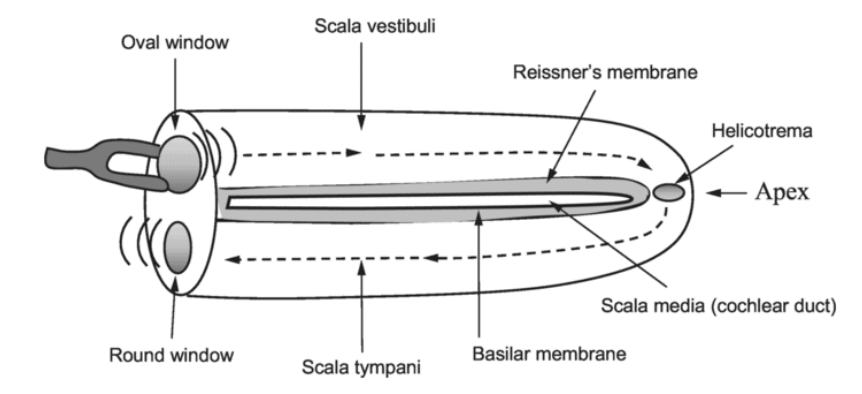
\includegraphics[width=\textwidth]{wayland-cohlear.png}
      \caption{'Unrolled' cohlear from \citet{Wayland2018Phonetics}}
      \label{fig:cohlear}
   \end{minipage}
   \hfill
   \begin{minipage}{0.48\textwidth}
      \centering
      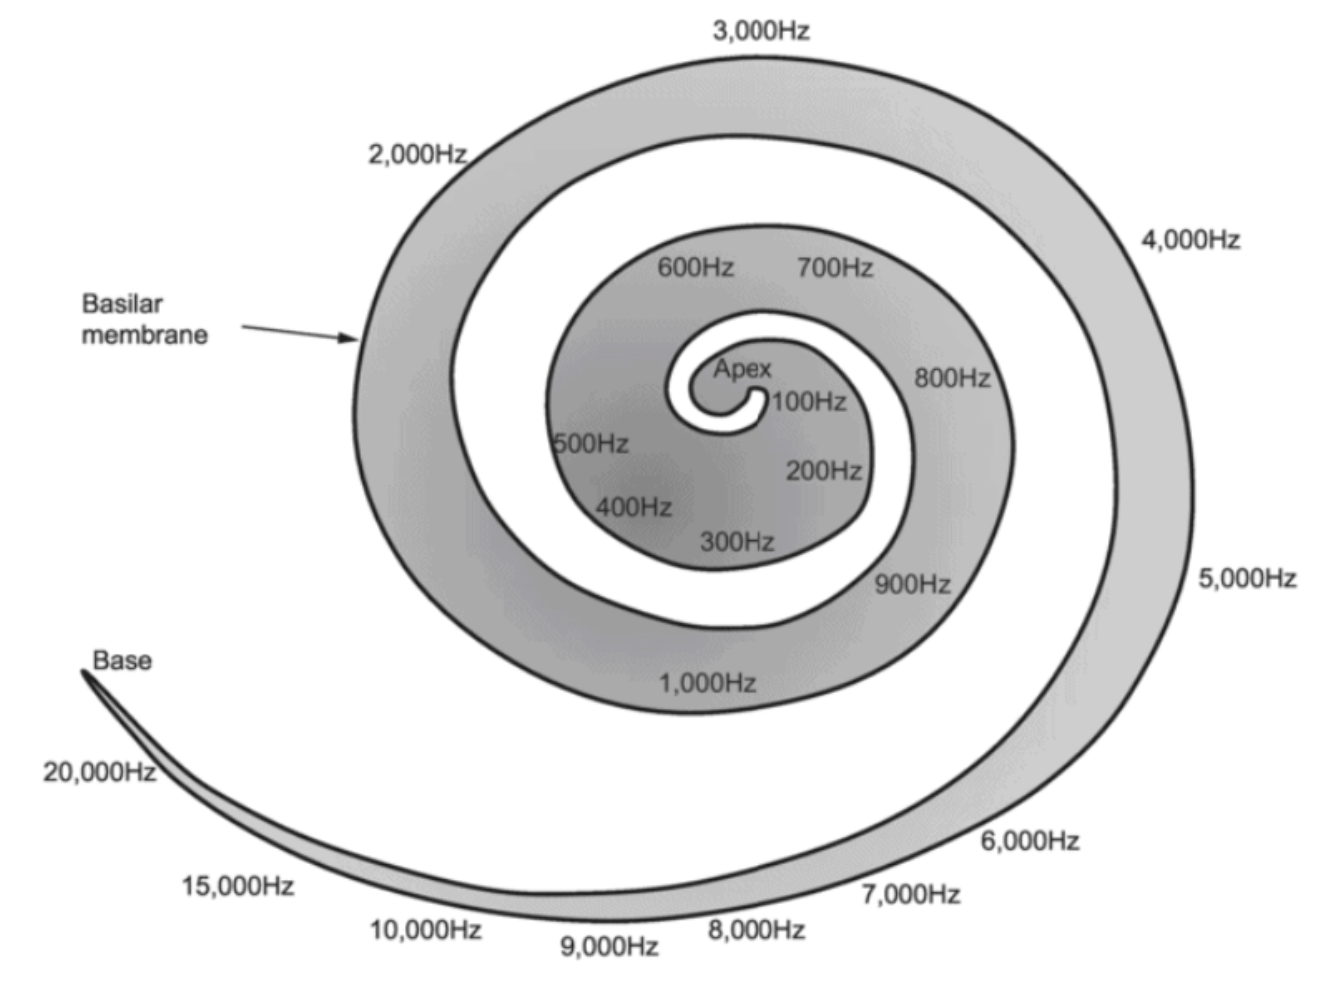
\includegraphics[width=0.5\textwidth]{wayland-corti-2.png}
      \caption{The Organ of Corti and the frequency responses. From \citet{Wayland2018Phonetics}}
      \label{fig:corti}
   \end{minipage}
\end{figure}

% \subsection{Congenital Hearing Loss}
% TODO
% \subsection{Exposure to Loud Noises}
% TODO
% \subsection{Ageing}
% TODO
\subsection{Hair Cell Loss and Hearing Loss}
As we have seen, the hair cells play a major role in allowing humans to register sound. Unfortunately,
it is the major cause of hearing loss since those hair cells are suspectible to damage.
The cause of hair cell loss is complex, since it could be due to many factors such as 
genetic abnormalities (congenital hearing loss), infection, diseases or extrinistic factors such as exposure to loud noises.
It can also occur due to aging, which could be due to the reasons mentioned above, but also 
could be triggered due to age related hearing loss genes. To make matters worse, hair cell loss is unrecoverable in humans \citep{Furness2015HairCell}.
Hearing loss is a spectrum, and varies from mild (26-40dB loss), moderate (41-60dB loss), severe (61-80dB loss) to profound($>80$dB loss) \citep{Nieman2020HearingLoss}.
Moreover, hearing loss may occur in one ear (unilateral) or in both ears (binaural). 

\section{Hearing Loss Treatment}

We now know how the auditory system works, and how hearing loss can occur.
Hearing solutions have come a long way, 
from acoustic devices to modern digital devices. 
As this dissertation is focused on 
the incorporation of machine learning techniques into hearing aids,
we will gloss over the history of acoustic devices, but 
for a comprehensive overview of the history of hearing technology,
refer to the paper by \citet{levitt_historical_2007}.

% \subsection{History of Hearing Technology}
% TODO: Will see how much pages I have left after doing other chapters.

% Users were fitted with what would have been considered a HA in this day and age as early as the 18th century.


\subsection{Hearing Technology}
As mentioned in the Introduction, the most common treatment for hearing loss 
is the provision of hearing technology. There are two common approaches 
to fitting of hearing technology: the equipment of a Hearing Aid (HA) 
or the fitting of a Cohlear Implant. There are similarities in the 
two, and both can be used to fit users that are experiencing profound hearing loss, 
though typically cohlear implants are only considered if the user is experiencing 
a severe hearing loss or further. While we 
focus on the HA, the concepts we explore can be applied to the CI.
The components of a HA vary widely, but at the very least, 
it contains a microphone, amplifier, receiver, and battery \citep{schuster-bruce_conventional_2025}.
A microphone is a device that converts acoustic sound waves into electrical signals. 
The electrical signals are then amplified by the amplifier, and the receiver converts the electrical 
signals back into the acoustic waves. The battery is used to power the device. 
Depending on the user, they may either be fitted with a hearing aid on each 
ear (binaural) or a single hearing aid on one ear (unilateral). 
Typically, the hearing aid contains multiple microphones, and the microphones 
are placed in different locations on the device. 
% Figure \ref{fig:hearing-aid} shows an image 
% of a hearing aid.


\subsection{Hearing Technology Now}

% Recent advances in hearing aid technology have led to the integration of increasingly sophisticated signal processing algorithms, including deep neural networks (DNNs) and artificial intelligence (AI), to enhance auditory performance and overall quality of life for users.
% High-profile innovations, such as Apple’s FDA-approved AirPods and developments from established manufacturers like Phonak and Oticon, exemplify this trend with the incorporation of DNN-based processing techniques.

% A notable development is the shift towards rechargeable hearing aids that utilise lithium-ion batteries.
% These devices not only offer the practical benefit of eliminating battery replacement but also support higher peak power consumption, thereby accommodating the computational demands of advanced models such as DNNs.
% In contrast, hearing aids powered by zinc-air batteries remain limited by the intrinsic energy constraints of their power source.
% Recent studies report that under high power conditions, the average battery life of non-rechargeable, zinc-air-powered hearing aids lies within the range of 50–80 hours \citep{sparkes_study_1997, mir_evaluation_2023, thomas_zincair_2024}.
% Rechargeable devices typically achieve operational durations of 15–30 hours, and when features like Phonak’s Speech Enhancer are activated in noisy environments, maximum battery life can drop to below six hours.


% These findings underscore a fundamental trade-off in hearing aid design: while the application of DNNs can significantly elevate the performance of auditory devices, it concurrently imposes strict energy requirements that may compromise battery longevity.
% Future research should therefore focus on optimising power efficiency to better balance computational performance with practical usability.

As discussed in the Introduction, the increasing demand for HAs is not only 
driving the development of more sophisticated HAs, but also the entry of big tech 
companies like Apple to the hearing aid market, and the developments from established 
manufacturers like Phonak who are starting to incorporate DNNs into their devices.

Another trend is that of the shift towards rechargable hearing aids (Lithium Ion Batteries).
These devices not only offer the practical benefit of eliminating battery replacement but also support higher peak power consumption 
which could explain the correlation in the sudden interest in using DNNs in HAs.
In contrast, hearing aids before the shift towards rechargable hearing aids were using Zinc-air batteries 
(\cite{sparkes_study_1997}; \cite{mir_evaluation_2023})
which are non-rechargable.
A recent study by \citet{thomas_zincair_2024} which 
experiments with various Zinc-air manufacturers, shows that the average battery life 
under high power conditions is 50-80 hours. Contrast this with the average battery life of 
rechargable hearing aids which is typically in the region of 15-30 hours and 
features such as Phonak's Speech Enhancer (the DNN based feature) can drop the battery life 
to below 6 hours. 

These findings highlight an important trade-off in hearing aid design: 
while there is loads of potential to improve the performance of HAs (DNNs or otherwise)
it can come at the cost of battery life and possibly constrains 
the types of models that can be used. NBASNSADNADNASDN

Due to the proprietary nature of the devices, it is unclear what sort of 
algorithms are used in the devices. Though, from Phonak's white paper on Spheric Speech Clarity \cite{Hasemann2024PhonakSphere}
we can deduce that the devices use a combination of ASA and speech enhancement techniques.
From the paper, before signal processing begins, the sound is fed into Autosense OS which 
performs 'scene classification' so in the context of this project, this can be 
considered as an acoustic scene analysis (ASA) algorithm. More specifically, if 
the signal is classified as 'Speech in Loud Noise', then the signal is fed into a 
deep neural network which outputs a mask that seperates the speech signal from the background noise 
which is then applied to the signal. 



% It is enough 
% to know for now that the devices will contain multiple microphones, and 
% a dedicated chip which does further processing on the sound depending 
% on the environment the user is faced with.
% It should be pointed out that there is an active area 
% of research into curing congenitial hearing loss - individuals who have been diagnosed with 
% a hearing loss since birth.
% \subsubsection{Hearing Aids}
% Figure ... shows a typical hearing aid, and Figure ... shows the hearing aid labelled.
% TODO
% Microphone info, the reason for multiple mics etc
% There is a surge into rechargable hearing aids.
% Smaller model = higher battery life 

% \subsection{New Approaches to Treatment}
% \subsubsection{Gene-Based Therapy}
% Genitic mutations account for 70-75\% of congenital hearing loss, and with the advent 
% of gene-based therapy, it is not surprising to see that this avenue is explored with hearing loss. 
% However, besides it being an active area of research, it will not be applicable 
% to individuals that have 

\newpage
\section{Speech Processing Techniques}
\subsection{Digitisation}
\begin{figure}[h]
   \centering
   \includegraphics[width=\textwidth]{waveform-spectrogram.png}
   \caption{A wavefrom (bottom) and its spectrogram (top). 
   We used an excerpt mixed with speech with the `InTraffic'
   environment from the HEAR-DS dataset \citep{Huwel2020HearDS}.}
   \label{fig:waveform-spectrogram}
\end{figure}
To be able to perform speech processing on a device containing a chip/processor such as a HA, requires us 
to have some sort of digital representation of the sound wave. A waveform is just that, a digital representation 
of the sound we hear [Figure \ref{fig:waveform-spectrogram}]. A microphone is a device that converts those sound waves into a representation of the 
waveform. Conceptually, this is done by measuring the relative air pressure at different points in time, and 
this is represented as a waveform or a time series of amplitudes. Digital devices can't have infinite precision, so the signal produced by the sound will 
be divided into discrete samples, and the rate at which this occurs is known as the sampling rate. Additionally,
the precision of the amplitude of the signal will be quantized into discrete numbers, and the precision is 
dictated by the bit depth (or the quantization rate).

The selection of these two parameters is determined by the nature of the speech task and the Nyquist-Shannon Sampling Theorem.
This theorem asserts that the sampling rate should be at least twice the highest frequency present in the signal. 
That is, for a signal containing frequencies up to 8KHz, the minimum required sampling rate would be $f_s \ge 16$KHz.
Otherwise, aliasing will occur, which is the phenomenon where high frequency components could be misinterpreted as lower frequencies,
which could be undesirable in both tasks we are trying to perform. Typically, datasets will have a sampling rate 
of 44KHz, and commonly for ASA tasks, a sampling rate of 16KHz is acceptable. 
Regarding the bit depth, it is selected based on the dynamic range required to capture speech signal variations. 
Commonly, 16-bit depth is used, which is capable of representing an amplitude range of approximately 96dB, thereby ensuring sufficient resolution in amplitude representation.

\subsection{Engineered Acoustic Features}
The prevalance of engineering acoustic features in previous work relating to my project and speech processing in general,
warrants a high level overview of this concept to better understand its usage. 
Given some signal $x(t)$, an engineered feature $f(x(t))$ is a function that transforms the signal in some way.
In this project we will be feeding the models the log mel spectrogram of the signal. To obtain the log mel spectrogram, 
we first need to convert the signal (waveform) into the frequency domain (spectrogram) [Figure \ref{fig:waveform-spectrogram}].
The process of converting the signal into the frequency domain is done by utilising 
the Fourier Transform. We will technically be using the Fast Fourier Transform (FFT) 
due to efficiency, and the main hyperparameters for the FFT are the window length $w$ 
and the hop length $h$. The window length is the length of the window that is used to 
split the signal into frames, and the hop length is the number of samples between the 
start of each frame. Additionally, there is a choice of a window function and we will 
be using the most common one, the Hann window. Once we apply the FFT, we will be 
left with a complex valued vector of length $w$ and the magnitude of this vector 
gives us the amplitude of the signal at different frequencies. 
We can then apply a Mel Filterbank - a filterbank that is used to mimic the human auditory system. 
Afterwards, we take the logarithm of the filterbank outputs and we are left with the log mel spectrogram 
which mimics the human perception of loudness. Diagram \ref{fig:log-mel-spectrogram} shows the process to make it more clear.

The reason it is worthwhile to use an engineered feature is for many reasons, but one of the main ones is that 
it is a compact representation of the signal which reduces the amount of memory and computational resources required 
to process the signal which is especially important for embedded devices such as HAs. 
Additionally, the log mel spectrogram enhances the distinction between speech and background noise, which 
may make a model more effective at ASA and speech enhancement tasks.
\section{Related Work}
As this project will chain two algorithms—Acoustic Speech Analysis (ASA) and Speech Enhancement, 
to form a state-dependent model, we will cover each task in separate sections. We also add 
a small section on how the idea of Green AI can be applied to the development of the models.

\subsection{Acoustic Scene Analysis (ASA)}
We will be using HEAR-DS dataset introduced by \citet{Huwel2020HearDS}. This dataset was developed in response to the inadequacies of existing ASA databases for HA processing. A more detailed description of the dataset is provided in Chapter \ref{sec:datasets}.
The original paper on the HEAR-DS dataset illustrates its applicability by employing a Convolutional Neural Network (CNN) for environment classification. In Chapter \ref{chap:acoustic-scene-classification}, an attempt is made to reproduce the results presented in that study. The challenges encountered during this replication process are discussed comprehensively in the chapter. Additionally, to validate the model implementation, the same parameters were applied to the DCASE 2017 Acoustic Scenes Challenge dataset \citep{DCASE2017challenge}. In particular, a comparison is drawn between the model proposed by \citet{schindler_multi-temporal_2018} and the CNN model used in the HEAR-DS paper, with the findings detailed in Section \ref{sec:DCASE-results}.
The two papers mentioned above utilise engineered features, and more specifically, the log mel spectrogram. This 
approach in some literature is called operating on the frequency domain. It is worth pointing out 
that there is research into doing ASA on the time domain i.e. operating on the waveform directly, 
such as the papers by \cite{dai_very_2016} and \cite{kumar_end_2020}. While not explored in this part, 
it is something I will look into exploring in part 2 of this dissertation as there is 
a compelling reason to possibly consider the time domain approach. Namely, 
the overhead of the Fourier Transform and the Mel Filterbank in a hearing aid 
is potentially too high, and so working directly with the waveform may be a more feasible approach.

% TODO: VERY DEEP CONVOLUTIONAL NEURAL NETWORKS FOR RAW WAVEFORMS

\subsection{Speech Enhancement}
On the other hand, Speech Enhancement aims to improve the perceptual quality of a speech signal that 
has been degraded by an additive noise \citep{loizou_speech_2007}. 
This enhancement is crucial in applications where speech intelligibility is essential, such as telecommunications, hearing aids, and speech recognition systems. Noise sources may include environmental disturbances (e.g., wind noise) as well as interference from multiple speakers (e.g., babble noise).

There are many different approaches to speech enhancement, from more traditional methods such as spectral subtraction, or Wiener filtering
to more modern methods that incorporate neural-networks. In this dissertation, we will be using a neural-network based approach.
But even within the neural-network based approach, there are different techniques that can be used to enhance the speech signal. 
Neural network-based speech enhancement algorithms can be categorised into four primary types, as described in \cite{katagiri_handbook_2000}:
\begin{itemize}
   \item \textbf{Time-Domain Filtering} - Trains a neural network with noisy inputs (background + speech) and clean targets (speech only). 
   This involves working with the waveform directly, however it is not without its challenges which is still an active area of research \citep{saleem_time_2024}.
   \item \textbf{Transform-Domain Filtering} - Trains a neural network with noisy inputs (background + speech) and clean targets (speech only). 
   The differnece between this and the Time-Domain Filtering approach is that the input is transformed into the frequency domain 
   (whether that be a Fourier Transform, or a Mel Spectrogram, Mel-Frequency Cepstral Coefficients (MFCCs), LPC, etc). The advantage of this 
   is that the dimensionality of the input is usually lower, and the representation is more robust to seperation of the speech and background noise.
   This is also a popular approach in the speech enhancement literature \citep{hou_local_2023}.
   \item \textbf{State-Dependent Model Switching} - The two mentioned approaches assumes that the speech signal and noise source are stationary. 
   This is too strong of an assumption, and so state-dependent model switching is a paradigm that has been explored. The main idea is 
   to have a class of models, each specialising in handling a different type of noise and to switch between them based on the 
   characteristics of the input signal. This in a way is the chaining of ASA and Speech Enhancement, as the ASA model will 
   first classify the input signal into a state, and then the appropriate speech enhancement model will be selected and applied to the signal.
   To our knowledge, this technique in the context of HAs has not been discussed in the literature but it 
   seems to be implemented in state-of-the-art HAs. 
   \item \textbf{Online Iterative Methods} - The focus is on incorporating adaptive techniques that do not rely on pre-existing 
   training data. Key approaches include adaptive predictors, dual EKF (Extended Kalman Filter) algorithms, and noise-regularised adaptive filtering.
   There is some active research into incorporating Kalman Filters (KFs) or EKFs into the neural pipeline for speech enhancement \citep{Xue2020NeuralKF},\citep{Mellahi2023SpeechEU}.
\end{itemize}
The discussion of the engineering of acoustic features in the previous section is relevant here, as the Transform-Domain Filtering approach
is what will be used in this part of the dissertation. 
Then, the main contribution of this dissertation is the exploration of 
the feasibility of state-dependent model switching in the context of HAs. 
Given that it seems to be already used in state-of-the-art HAs, it 
would be a good idea to formalise this approach in the literature 
so that potentially future work can build on this.


% Though, exploring the time domain approach is something I will be looking into for the second part of this dissertation 
% due to the potential overhead reduction of the time domain approach as mentioned in the previous section.

\subsection{The parallels of Green AI}
The paper by \citet{schwartz2019greenai} discusses the idea of Green AI 
which is to advocate for the use of hardware-independent performance metrics.
Metrics such as electricity consumption or elapsed real time are not good metrics 
as they are dependent on the hardware on which the model is run. 
Although the number of parameters in a model has been proposed as an 
alternative metric, it can be problematic when comparing different model architectures 
since it is possible that despite a more complex model having more parameters, 
it could compute the same amount of work in a more efficient manner. 

Instead, \citet{schwartz2019greenai} discusses how the number of floating point operations (FLOPs)
provides a more concrete and meaningful measure of computational workload. 
FLOPS are computed by analytically counting the number of \texttt{ADD} and \texttt{MULT} operations in the model.
This is effective, as all operations in a DNN can be recursively reduced to a combination 
of \texttt{ADD} and \texttt{MULT} operations.
As an added bonus, the fact that we have an insight into HA's potential FLOPs is useful 
as it allows us to compare the model's performance to the hardware's potential. If our 
models are using less FLOPs than a HA device, then we know that the model is 
potentially more energy efficient or that we could investigate expanding 
the model. On the flip-side, if the model is using more FLOPs than a HA device, 
then we know that the model is potentially too large for a HA device and we need 
to look for ways to reduce the model size. It also helps that there is load 
of literature on reducing the FLOPs of DNNs (e.g. \cite{liu_simple_2023}) so 
using FLOPs as a metric is not only good from a reproducibility standpoint, 
but from a development standpoint as well. 

\section{Criticism of Previous Work}
We found out that the paper by \citet{Huwel2020HearDS} had 
some issues which prompted us to do a more thorough analysis of the ASA 
model they presented. Granted, the paper was more of an exploration of the applicability of the dataset rather than a thorough analysis of the 
performance of the model, there was some issues with 
the results and gaps in the analysis which we aim to address in this part of the dissertation. 
Additionally, as will become clear, the reproduction of the results 
was difficult and while we had to deviate from the paper's approach 
in some aspects, in other cases, we had to make some assumptions 
about the pipeline details of the paper.

As the dataset is very likely to not be balanced, (as will become more clear in Chapter \ref{chap:acoustic-scene-classification})
it was an odd decision for the authors 
not to talk in detail about the splitting strategy of the dataset 
and how they handled the imbalance. In particular, the metric 
for the accuracies was what we believe to be quite a 
naive approach to evaluating the model's performance (a simple accuracy score).
It would have also been more informative to see how the model performs at various 
SNRs (Signal-to-Noise Ratio) since it is possible that the model is performing poorly at low SNRs.
So we will be extending the evaluation of the models to include these aspects. 
More so, we will also incorporate precision, recall and F1 scores to get a more 
holistic view of the model's performance. 

Reproduction issues aside, the paper concludes that the 
most complex model was able to compute the environment 
with a latency of 0.4s. However, the paper uses 
a computer-powered device to run the model, which 
could potentially be more powerful than a HA device. 
We will be taking a more thorough approach to
investigating the viability of the models when used in a HA device 
and be reporting FLOPs as per \citet{schwartz2019greenai}.
The paper does mention that more verbose evaluation was not 
the scope of the paper, and so this dissertation aims 
to bring more insight into the viability of the models 
when used in a HA device.

It is important to note that the intention is not to 
be critical of the original authors, but rather to 
bring more insight that was built from the work of the original authors.
This is done by providing a deeper insight into the model's performance 
and feasibility when used in a HA device. The challenges encountered 
in reproducing the results underscore the need for more 
detailed methodological documentation, and so this dissertation aims 
to address this gap.

In summary, while the previous study makes a valuable contribution
to the field of HA research, a more thorough and systematic
evaluation is necessary to fully assess the model's efficacy 
in the task of ASA. This dissertation aims to contribute 
to that venture by offering a comprehensive analysis
of the model under conditions that more closely mirror real-world HA applications.
Additionally, we want to take the paper's mission further and explore 
other use-cases of the dataset, such as the task of Speech Enhancement 
and how the two tasks (ASA and SE) can be combined to form a state-dependent model,
all within the context of a HA device.

% and CHiMe 5 \cite{barker18_fifth_2018} datasets. However, only the CHiME 3 development set was used for mixing the speech into the background noise.
% CHiME 5 was used for creating a new environment, 'Interferring Speakers', which are samples that contain speech from multiple speakers.
% I think using the CHiME 3 dataset and especially only the development set was an odd decision, as there is only roughly 10 hours of data 
% from 4 speakers. So a model trained on this dataset may not generalise well to real world scenarios, due to the rich variability of 
% speech from different speakers. Nevertheless, we continue with the paper's approach to set up a baseline. Another odd decision was 
% in the use of a fixed learning rate scheduler, and the use of a high epoch count without what appears to be no early stopping. This 
% will be discussed in more detail in Chapter \ref{chap:acoustic-scene-classification}. We still thank the authors for their work on the dataset 
% as it is a promising dataset for the future of HA research. Additionally, given that the dataset 
% has the potential to be used for HA devices, there is not any mention on the viability of the models 
% when used in a HA device. So a significant aspect of this project is to investigate the feasibility of 
% incorporating a DNN model into a HA device. 


\chapter{Methodology}

% The model presented in the paper assumed a sampling rate of 16KHz, so we resampled the HEAR-DS dataset to 16KHz. Additionally, 
% the model expected a log-mel spectrogram of 10s segments, and the HEAR-DS dataset provided longer segments. We therefore 
% split the HEAR-DS segments into 10s segments by traversing the dataset and extracting 10s segments. There is potential 
% for this to have discontinuities in the beginning and end of the segments, but from the paper it is unclear how this 
% was addressed if at all. We went with a naive approach of just cutting the segments.


\section{Acoustic Scene Analysis}
\label{sec:methodology-asa}
Mathematically, ASA can be formalised as follows:
Consider an audio signal \(x \in \mathbb{R}^{T}\), where \(T\) denotes the number of samples in the signal, and let \(\mathcal{E} = \{e_1, e_2, \ldots, e_N\}\) represent a set of \(N\) distinct environments. ASA is concerned with determining a mapping 
\[
f: \mathbb{R}^{T} \rightarrow \mathcal{E},
\]
which assigns each audio signal to one of the environments in \(\mathcal{E}\). In this project, \(f\) is implemented as a neural network
and in this first part of the dissertation, we will be using a Convolutional Neural Network (CNN) to implement \(f\).

\subsection{Model}
\label{sec:asa-model}
\begin{table}[h]
   \centering
   \begin{tabular}{|c|c|c|c|}
      \hline
      Model & $CNN_1$ & $CNN_2$ & $FC$ \\
      \hline
      net-8 & 8 & 16 & 25 \\
      net-20 & 20 & 40 & 63 \\
      net-32 & 32 & 64 & 100 \\
      \hline
   \end{tabular}
   \caption{Model parameters for the net-X models.}
   \label{tab:cnn-model-params}
\end{table}
As our baseline model, we will be using the CNN model presented in the paper by \citet{Huwel2020HearDS}. 
The model has three hyperparameters: the number of output channels for the first and second convolutional layers ($CNN_1$ and $CNN_2$),
and the number of neurons in the fully connected layer ($FC$). The researchers investigated the effect of different model parameters, 
and in the paper, they train the dataset on 7 different models, where they vary the number of output channels in intervals of 4, thereby training 7 different models.
Due to the time constraints, we will be training 3 models, as we're mostly interested in seeing if we're getting similar results to the paper.
Table \ref{tab:cnn-model-params} shows the parameters of the models we will be training.

The model architecture is shown in Figure \ref{fig:cnn-model-architecture}. As 
mentioned earlier the models operate on the frequency domain, and 
we stuck with the paper's approach of using a Mel Spectrogram as the 
frequency domain representation for reasons mentioned in the background section. 
As per the paper, all the convulaotional layers use a $7 \times 7$ kernel
with a stride of $1 \times 1$ and padding of $3 \times 3$. After the convoluational operation, 
batch normalisation is applied which can help with the stability of forward propagation 
and can act as a regulariser which can help prevent overfitting \citep{prince2023understanding}.
The choice of activation function is a Rectified Linear Unit (ReLU) which is computionally 
efficient and reduces the risk of the vanishing gradient problem \citep{prince2023understanding}.
As the preceding operations can increase the dimensionality of the input, a form of down-sampling is applied by using a max-pooling operation which helps in achieving 
translation invariance and reducing computational complexity for the following layers. Something worth considering for 
part 2 of this dissertation is to explore the use of other down-sampling techniques, and in particular,
\citet{liu_simple_2023} have proposed a family of simple pooling front-ends (SimPFs) 
which in some cases reduce the number of FLOPs as much as 75\% in acoustic scene classification tasks. 
Lastly, dropout of 0.3 is applied after the max-pooling operation which can help with 
the model generalisation \citep{prince2023understanding}.
Applying convolutions is not enough for ASA, 
as we need to have a way to compare the output of the CNN with the set of environments \(\mathcal{E}\).
This is where the fully connected layer comes in, as it will output a vector of size \(N\), where \(N\) is the number of environments.
The values of the vectors are logits, and so during training and inference, we use a softmax function to convert them into probabilities.
The softmax function is defined as follows:
\[
\sigma(x_i) = \frac{\exp(x_i)}{\sum_{j=1}^{N} \exp(x_j)},
\]
where \(x_i\) is the \(i\)-th element of the vector.
The environment with the highest probability is then chosen as the predicted environment 
i.e. \(\hat{e} = \arg\max_{e_i \in \mathcal{E}} \sigma(x_i)\).


\begin{figure}[h]
   \centering
   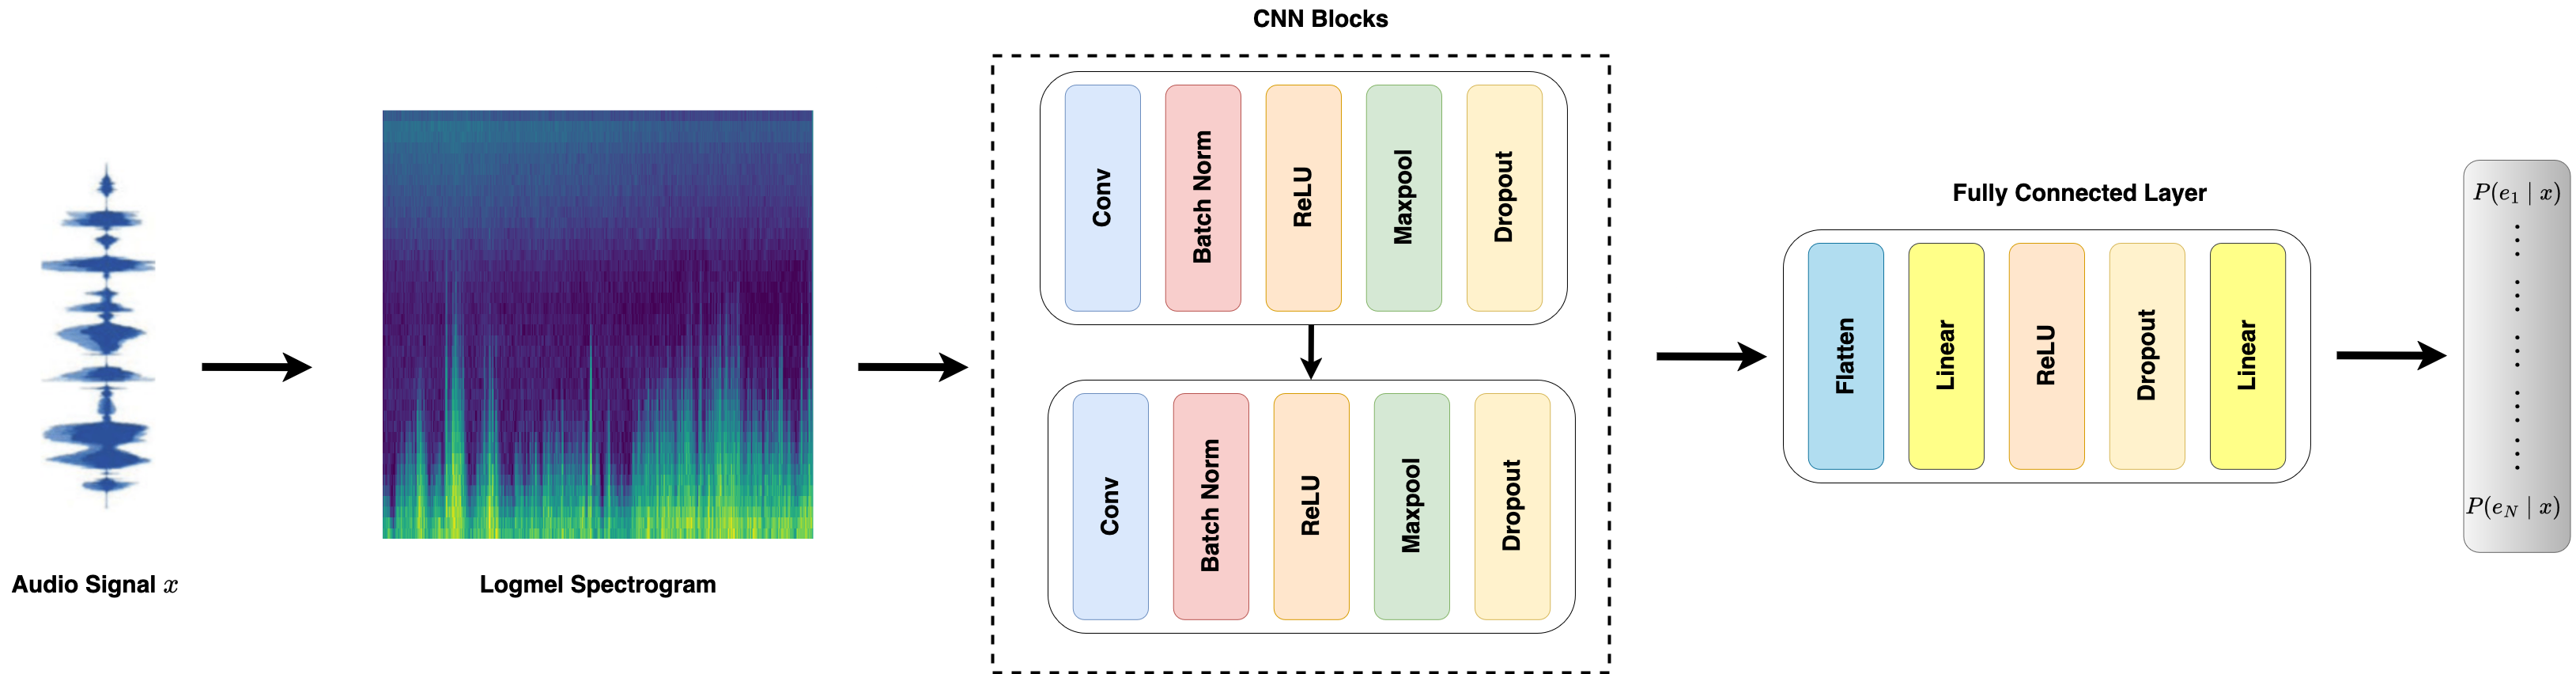
\includegraphics[width=0.95\textwidth]{cnn-diagram.png}
   \caption{The baseline ASA model architecture.}
   \label{fig:cnn-model-architecture}
\end{figure}

\subsection{Training}
For ASA, we need to have a dataset that contains audio signals along with their corresponding environmental labels. 
Mathematically, we need to have a dataset of the form \(\mathcal{D} = \{(x_i, y_i)\}_{i=1}^{N}\), where \(x_i \in \mathbb{R}^{T}\) is the audio signal, and \(y_i \in \mathcal{E}\) is the environmental label.
Then a loss function is needed to steer the model towards the correct mapping.
It is important to note that the dataset $\mathcal{D}$ is not necessarily balanced,
meaning that some environments may have more samples than others.
This is a problem, as the model may learn to classify all samples as the most frequent class. 
So to combat this, when using a loss function, we apply a weight to each sample based on the number of samples in the dataset.
The weight is defined as follows:
\[
w_i = \frac{n_{samples}}{n_{classes} \cdot n_i}
\]
where \(n_{samples}\) is the total number of samples, \(n_{classes}\) is the number of unique classes, and \(n_i\) is the number of samples in the \(i\)-th environment.
This balanced weighting scheme ensures that the weights sum up to \(n_{samples}/n_{classes}\).
So a vector of weights \(\mathbf{w} \in \mathbb{R}^{N}\) is created, where \(N\) is the number of environments
So we have a vector of weights \(\mathbf{w} \in \mathbb{R}^{N}\) which we can use to weight the loss function accordingly.
This is consistent with the paper by \citet{Huwel2020HearDS} where they did ``weighted update steps for each target environment depending on the number of samples in each environment.''
On the topic of the loss function, the paper by \citet{Huwel2020HearDS} does 
not explicitly mention the loss function they used, but we assume that they used the weighted cross-entropy loss function.
The weighted cross-entropy loss function is defined as follows:
\[
L(y, \hat{y}) = -\sum_{i=1}^{N} w_i \cdot y_i \log(\hat{y}_i),
\]
where \(y_i\) is the one-hot encoded environmental label, and \(\hat{y}_i\) is the predicted probability of the model.

Once we have the loss function, we can use it to train the model. There are many approaches to training a model,
and for reproducibility (and as a baseline), we will be using the paper's approach of using Stochastic Gradient Descent (SGD) with a fixed learning rate.
The learning rate was decreased every 40 epochs in a quasi-logarithmic manner: [0.05, 0.01, 0.001, 0.0005, 0.0002, 0.0001].
This leads to a total of 240 epochs of training. 
However one of objectives of this part of the dissertation was to explore if a different approach to learning rate scheduling
could yield better results. So we will be exploring a different approach to learning rate scheduling in the experiments.
It will be found that the Adam optimiser converges faster than the SGD optimiser and still results in a comparable 
performance. 
\subsection{Evaluation}
The evaluation of the ASA model will be done with a few metrics. 
We will adopt the accuracy metric which is something the paper by \citet{Huwel2020HearDS} also used.
The accuracy is defined as follows:
\[
Accuracy = \frac{1}{N} \sum_{i=1}^{N} \mathbb{I}(y_i = \hat{y}_i),
\]
where \(N\) is the total number of samples, \(y_i\) is the one-hot encoded environmental label, and \(\hat{y}_i\) is the predicted environmental label
and \(\mathbb{I}\) is the indicator function which is a piecewise function that returns 1 if the condition is true and 0 otherwise.

However, the issue with accuracy is that taking it 
at face value can be misleading, even more so in the case of an imbalanced dataset 
which as will become clear when we discuss the dataset in Chapter \ref{chap:dataset},
this is certainly the case for the HEAR-DS dataset. 
So on top of the accuracy metric, we will also be using precision, recall and F1 score metrics.
These metrics are defined as follows:
\[
Precision = \frac{TP}{TP + FP},
\]
\[
Recall = \frac{TP}{TP + FN},
\] 
\[
F1 = 2 \cdot \frac{Precision \cdot Recall}{Precision + Recall},
\]
where TP is the number of true positives, FP is the number of false positives, and FN is the number of false negatives.
Intuitively, precision is how well the model is doing at correctly identifying the positive class,
while recall is how well the model is doing at correctly identifying all positive samples.
The F1 score is the harmonic mean of precision and recall.

Another aspect that we will be looking at is how the models peform at various SNRs. 
This is because given some noisy sample, the model may perform differently depending on the SNR of the sample.
It will be interesting to see how the model performs at the lowest SNR,
as this is where the speech is quite faint and the background noise is quite strong. 
Given that the model we will be training uses background and background+speech environments,
it is possible that the model may conflate the two classes at the lowest SNRs.


From a feasibility perspective, we will be adopting the Green AI principles \citep{schwartz2019greenai} 
and evaluating the model using the following metrics:
\begin{itemize}
   \item \textbf{Floating Point Operations (FLOPs)}/\textbf{Multiply Accumulate (MACs)} - This will be done by looking at the number of operations the model performs.
   \item \textbf{Number of Parameters} - This will be done by looking at the number of trainable parameters in the model.
\end{itemize}

\section{Speech Enhancement}
\label{sec:methodology-se}
\begin{figure}[h]
   \centering
   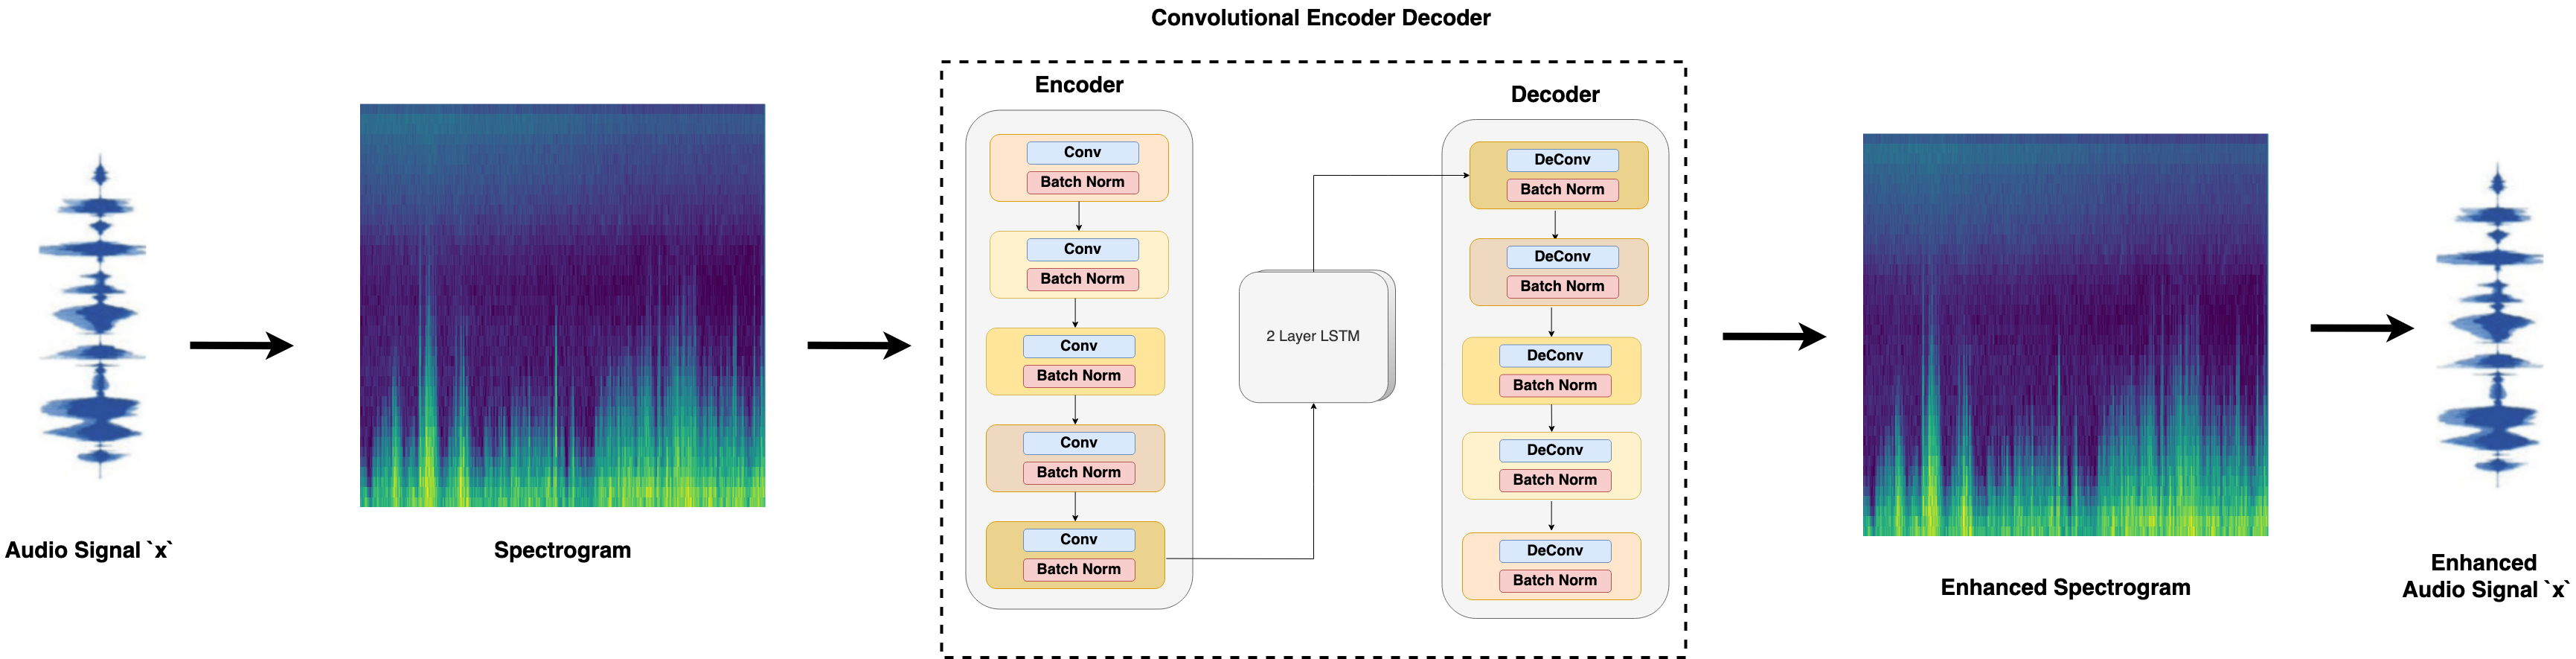
\includegraphics[width=0.95\textwidth]{se-model-diagram.png}
   \caption{The speech enhancement model architecture.}
   \label{fig:speech-enhancement-model-architecture}
\end{figure}
Mathematically, let a noisy speech signal be represented by \(x \in \mathbb{R}^{T}\) and the corresponding clean speech signal by \(y \in \mathbb{R}^{T}\), where \(T\) denotes the total number of samples.
Speech enhancement is therefore concerned with determining a mapping 
\[
f: \mathbb{R}^{T} \to \mathbb{R}^{T},
\]
which takes a noisy speech signal \(x\) and produces an enhanced version \(f(x)\) that is as close as possible to the clean speech signal \(y\) i.e.
\[
f(x) \approx y.
\]
Just as in the previous section, we will be using a Convolutional Neural Network (CNN) to implement \(f\).
\subsection{Model}
\label{sec:se-model}
As this is more of an exploration of the viability of using a DNN model for speech enhancement 
and the establishment of a baseline which can be used to improve upon, we will start 
with a simple 5-layer CNN model. The model is shown in Figure \ref{fig:speech-enhancement-model-architecture}.
As we want to preserve the dimensionality of the input, we 
have removed batch normalisation and pooling layers.
For similar reasons, we have set the padding to $1\times 1$ which ensures that the output has the same dimensionality as the input
and the kernel size is set to $3\times 3$. We kept the activation function as a ReLU.
Since this model has 5 layers, it has 5 hyperparameters: the number of output channels for each layer ($C_1, C_2, C_3, C_4, C_5$).
Table \ref{tab:speech-enhancement-model-params} shows the parameters of the model.

\begin{table}[h]
   \centering
   \begin{tabular}{|c|c|}
      \hline
      Layer & Output Channels \\
      \hline
      $C_1$ & 64 \\
      $C_2$ & 128 \\
      $C_3$ & 64 \\
      $C_4$ & 32 \\
      $C_5$ & 40 \\
      \hline
   \end{tabular}
   \caption{Model parameters for the speech enhancement model.}
   \label{tab:speech-enhancement-model-params}
\end{table}

It is worth noting that the output of the model is a complex spectrogram, which would 
not be suitable for a HA device. So we need to convert the output back to the time domain. 
There are two approaches that we have seen in the literature:
\begin{itemize}
   \item \textbf{Inverse Short-Time Fourier Transform (ISTFT)} - As the name suggests, this approach takes the inverse of the Short-Time Fourier Transform (STFT) of the input signal.
   So the input is a magnitude and phase spectrogram, and the output is a time domain signal. 
   \item \textbf{Griffin-Lim} - This is an iterative algorithm that estimates the phase of the signal just from the magnitude spectrogram alone. 
\end{itemize}
For the purposes of this dissertation, the Griffin-Lim approach was adopted, as the initial implementation did not track phase information however,
it is something that we may explore in the future.


\subsection{Training}
We will adopt the Adam optimiser instead of SGD as one of the experiments I will be doing 
is to validate if the claim made in \citet{Huwel2020HearDS} that a fixed learning rate SGD approach
is better than an Adam optimiser approach. As will be discussed in Chapter \ref{} 
we found that the Adam optimiser converged faster than the SGD optimiser and still resulted in a comparable 
performance. Additionally, from the ASA experiments, we also found that adopting an early stopping criterion 
once the training loss plateaued, sped up the training process at no loss of performance. So we will be adopting 
this approach for the speech enhancement experiments as well. More specifically, we will be using a learning rate of $0.001$
and early stopping once the training loss stops improving after 5 epochs.

The way the model is trained is by comparing the ground truth speech signal with the enhanced speech signal. 
As such, we have used the Mean Squared Error (MSE) loss function to train the model. The loss function is defined as follows:
\[
L(y, \hat{y}) = \frac{1}{T} \sum_{t=1}^{T} (y_t - \hat{y}_t)^2,
\]
where \(y_t\) is the ground truth speech signal and \(\hat{y}_t\) is the enhanced speech signal.
For model stability we have ensured that the spectrograms are normalised to have zero mean and unit variance.
This normalisation ensures that the loss function operates within a range from 0 (optimal) to 1 (suboptimal).

\subsection{Evaluation}
The evaluation of the speech enhancement model in this part of the dissertation will be 
done by assessing two artificial metrics. The other approach to evaluation is 
to use subjective listening tests, which is a gold standard for evaluating speech enhancement models.
However, as with all gold standard methods, they are time consuming and expensive to conduct. 
Artificial metrics aim to be a proxy for the gold standard methods. 

Firstly, the Short-Time Objective Intelligibility (STOI) \citep{taal_algorithm_2011} metric will be used to assess the intelligibility of the enhanced speech signal.
It is a function of the noisy speech signal $s_n$ and the degraded speech signal $s_d$ after enhancement.
The STOI metric computes a value in the range \([0, 1]\), which can be interpreted as an approximation of the average percentage of correctly understood words in $s_d$. 
For the sake of brevity, we will not be going into the details of the STOI metric, but for interested reader, we refer them to \citet{taal_algorithm_2011}.

Secondly, the Perceptual Evaluation of Speech Quality (PESQ) \citep{rix_perceptual_2001} metric will be 
used to assess the perceptual quality of the enhanced speech signal. 
This metric is a function of the clean speech signal $s_c$ and the enhanced speech signal $\hat{s}_e$.
PESQ compares $s_c$ and $\hat{s}_e$, yielding a score between 1 (indicating poor quality) and 4.5 (indicating near distortion-free quality). 
As with STOI, the intricate details of the PESQ metric are not discussed here; the reader is encouraged to consult \citet{rix_perceptual_2001} for a comprehensive description.

A valid question to ask is why the model is not trained to directly optimise for both metrics. The primary challenge lies in the fact that both STOI and PESQ are non-differentiable,
which is a problem for gradient-based optimisation frameworks. However, there are methods to approximate the gradients of non-differentiable functions, and it is an active area of research.
For future work, this avenue may be explored. 

\section{Laying the Groundwork for State-Dependent Models}
\begin{figure}[h] \centering
   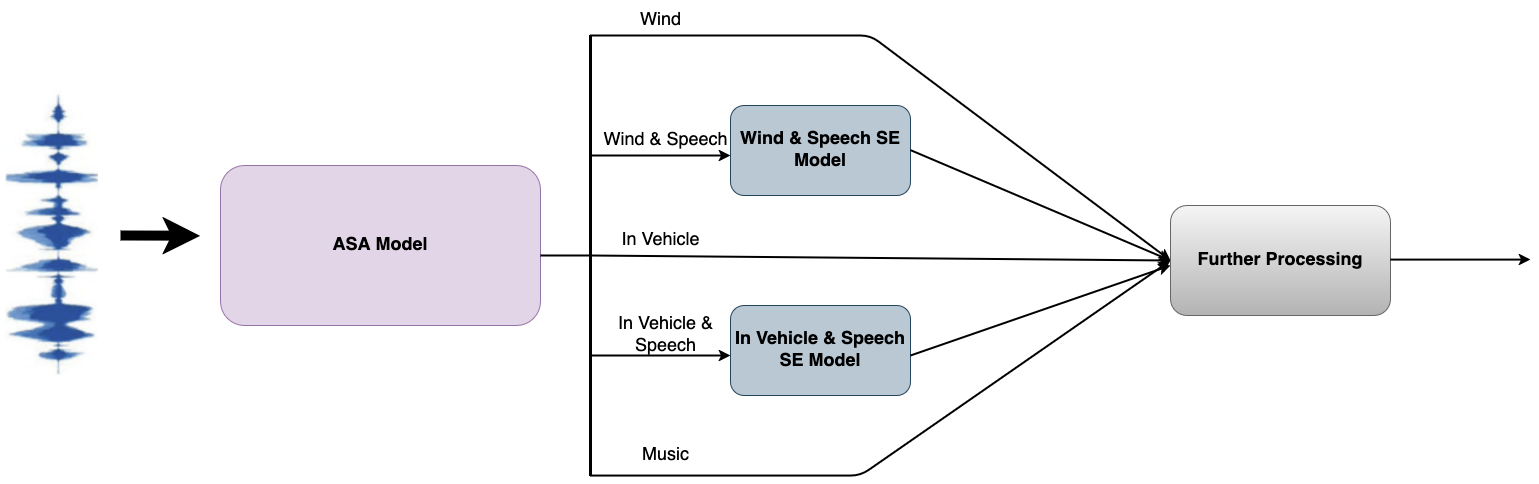
\includegraphics[width=0.9\textwidth]{state-model-diagram.png}
   \caption{The vision we have for the state-dependent model.}
   \label{fig:state-dependent-model}
\end{figure}
In the preceding sections, we have established the groundwork for the two tasks that we will be doing in this part of the dissertation.
The reason we are devising these two tasks in the first place is to set the groundwork for the next part of the dissertation which 
will be focused on the implementation of a state-dependent model. We hypothesise that a feasible state-dependent model can be created 
by chaining the two models together. Figure \ref{fig:state-dependent-model} shows the vision we have for the state-dependent model 
of which we aim to implement in the next part of the dissertation.
Mathematically, the state-dependent model can be represented as follows:
\[
f: \mathbb{R}^{T} \to \mathbb{R}^{T},
\]
where \(T\) denotes the total number of samples. 
Then, given a ASA model $g : \mathbb{R}^{T} \to \mathcal{E}$ and a family of SE models $h_{\epsilon} : \mathbb{R}^{T} \to \mathbb{R}^{T}$ for all $\epsilon \in \mathcal{E}$, 
$f$ can be represented as a piecewise function:
\begin{equation}
   f(x) = 
   \begin{cases} 
      h_{\epsilon}(x) & \text{if } g(x) = \epsilon \\
      x & \text{otherwise}
   \end{cases}
\end{equation}
In other words, the state-dependent model $f$ will apply the SE model $h_{\epsilon}$ to the input $x$ if the ASA model $g$ maps $x$ to $\epsilon$.
For example, if a HA user is situated in anenvironment characterised as `Wind Turbulence and Speech',
the state-dependent model will invoke the SE model that has been trained on this scenario to enhance the input signal $x$.
The state-dependant model is inspired by the unveiling of the Spheric Clarity DNN model by Phonak \cite{Hasemann2024PhonakSphere} in late 2024
in which if the HA user is faced in a 'Speech in Loud Noise' environment, the input signal $x$ will be passed through their Spheric Clarity DNN model.


\chapter{Experimental Setup}
\label{chap:experimental_setup}
With the methodological foundation laid out in the preceding chapters, we can now outline the hypotheses we aim to validate.
While we hinted at some of those hypotheses in the preceding chapters and sections, as a means of clarity, 
we will be outlining the hypotheses again here and in more detail so that the reader can have a comprehensive understanding of 
both the objectives and the rationale behind the experiments we will be doing.
Once we outline the hypotheses, another section is dedicated towards the datasets that will be used to validate the hypotheses.
Once that's done, the reader will be in a position to now analyse the results of the experiments which will be presented in Chapters \ref{} and \ref{}.
\section{Hypotheses}
\label{sec:hypotheses}
\begin{enumerate}
   \item \textbf{Replication of ASA Results.} 
   We hypothesise that the results reported by \citet{Huwel2020HearDS} for the ASA task can be replicated using the methodological approach detailed in Section \ref{sec:methodology-asa}.
   Achieving replication is crucial as it brings us a step closer to our vision of creating a state-dependent model in the next part of the dissertation.
   % TODO: Ask Hao if I should rephrase this to reject Huwel's claim that SGD is better than Adam due to weight initialisation issues?
   \item \textbf{Effectiveness of Utterance-Level Data Augmentation}. We hypothesise 
   that if we mix the speech signal with SNR at an utterance level, we will be able 
   to reduce the training time of the model and have similar performance to that of using 
   every SNR level per epoch. 
   Once again validating this hypothesis will speed up the development process going forward, 
   since if true, there will be less samples per epoch and thus less training time. 
   \item \textbf{Capability of the Speech Enhancement Model}.
   We hypothesise that the methodological approach detailed in Section \ref{sec:se-model} to 
   create a speech enhancement model will be able to enhance the speech signal by 
   cutting out the background noise. 
   \item \textbf{Superiority of State-Specific Training}
   As the end-goal of this dissertation is to create a state-dependent model, we hypothesise that
   training a model on each environment will result in a better performing model than training on all environments.
   We believe this could be due to the fact that with a shallower model, the parameters of the models 
   are less likely to be able to be fitted in such a way that all environments are catered for. 
   \item \textbf{Feasibility of Deployment on Hearing Aid Devices}.
   With the evaluation of the models with respect to the number of FLOPs and the size of the models,
   we aim to show that the models we implement are able to be deployed on HA devices. 
   This is a really important hypothesis to validate, otherwise any work 
   we do would not allow us to create a state-dependent model if the dependant models 
   are not able to be deployed on HA devices. (implication)
   \item \textbf{Comparative Performance of the Adam Optimiser.}
   It is hypothesised that using the Adam optimiser will result in a faster convergence with comparable performance to that of using a fixed learning rate Stochastic Gradient Descent (SGD) method, as employed in \citet{Huwel2020HearDS}.
   Validating this hypothesis will speed up the development process going forward, 
   enabling uniformity across subsequent experimental iterations. Additionally,
   it will allow us to reach the objective of creating a state-dependent model faster due to acceleration of the development process.
\end{enumerate}

\section{Datasets}
\label{sec:datasets}

\begin{table}[h]
   \centering
   \begin{tabular}{|c|c|c|c|}
      \hline
      Dataset & \rotatebox{90}{Environments} & \rotatebox{90}{No. of Speakers} & \rotatebox{90}{Hours of Data} \\
      \hline
   HEAR-DS \cite{Huwel2020HearDS} & 6 & - & 21 hours \\ % TODO: The hours is wrong, find the correct number
      CHiME 3 (booth dev. set) \cite{barker_third_2015} & - & 4 & 10 hours \\
      CHiME 6 (train + dev + eval) \cite{barker18_fifth_2018} & - & 48 & 50 hours \\
      TUT Acoustic Scenes 2016 \cite{mesaros_tut_2016} & 10 & - & 10 hours \\
      \hline
   \end{tabular}
   \caption{Dataset statistics.}
   \label{tab:dataset-stats}
\end{table}

\subsection{HEAR-DS}
\label{sec:hear-ds}
Given how much this dissertation revolves around the HEAR-DS dataset, we dedicate a section solely 
to the dataset. 
HEAR-DS is a dataset created by \citet{Huwel2020HearDS} which is specially tailored for Hearing Aid (HA) research. 
It consists of recordings captured on a dummy head equipped with Pinnae models and three microphones per side: one In-The-Canal (ITC) [in the ear] and two Behind-The-Ear (BTE) microphones (front and rear).
Each sample is recorded in either the left or right channel and decomposed into its respective microphone channels (BTE\_front, BTE\_rear, ITC), available in 48kHz/32bit format.
In the paper, the researchers used only the ITC samples, so for the scope of this project, we will only use the ITC samples as well. 
As the researchers were based in Germany, any recordings that they took were situated in Germany.
The dataset provides 7 environments:
\begin{itemize}
   \item \textbf{Cocktail Party} - Covers situations such as multiple speakers in a noisy environment or 'babble' noise. The paper mentions that this was mimicked by recording them in a university cafeteria or at a senior citizens' meeting.
   \item \textbf{Wind Turbulence} - Concerns the sound that is produced when wind passes through a microphone.
   \item \textbf{In-Traffic} - Samples where traffic noise is dominant such as bus stations or sidewalks. The researchers controlled for this environment to not be similar to the \textit{Wind Turbulence} environment by choosing 'calm' days for the recordings.
   \item \textbf{In-Vehicle} - The sounds produced when seated inside a car. The researchers controlled for this environment to not be similar to the \textit{In-Traffic} or \textit{Wind Turbulence} environments by ensuring the windows were closed. 
   \item \textbf{Quiet Indoors} - Mimic noises produced in a typical household such as washing dishes, clock ticking, etc. The researchers controlled for variability by recording the samples in several flats (rural, city centre, etc).
   \item \textbf{Reveberant} - Samples in highly reverberant environments such as a railway station hall, staircases or a church. 
   \item \textbf{Music} - The data is actually taken from the GTZAN dataset \cite{tzanetakis_musical_2002} and is used to test the model's ability to classify music.
\end{itemize}
Additionally, the researchers artificially created a new environment, \textit{Interfering Speakers}, which are samples that contain speech from multiple speakers. 
This is done by taking speech samples from the CHiME 5 dataset \cite{barker18_fifth_2018}. This environment is supposed to mimic the 
typical conversational speech that occurs in a real-world scenario. We however, decided to use the CHiME 6 dataset which 
supercedes the CHiME 5 dataset \cite{barker18_fifth_2018} by correcting the alignment of audio channels and the researchers 
recommend the use of the CHiME 6 dataset instead of CHiME 5 for any new research so we will use that instead. This could 
be an important factor as the methodology of creating the \textit{Interfering Speakers} environment is by finding 10s 
segments of speech that contain multiple speakers, so if the alignment of audio channels is not correct, the recordings 
may have a delay between the left and right channels which could have potentialy affected the results of the paper. We will discuss the dataset in more detail in section \ref{}.
In any case, the way this environment was created is unclear from the paper, but we do the following approach to create the environment:
\begin{enumerate}
   \item The code processes CHiME6 sessions to find 10-second segments containing overlapping speech from multiple speakers.
   \item For each segment, it extracts audio from the reference speaker's microphone and saves both left and right channels.
\end{enumerate}

To prevent the model from overfitting and increase the diversity of the data, the researchers provided multiple REC-SITs (Recording Situations) for each environment.
In the case of the \textit{Music} environment, each REC-SIT represents a different genre of music. This has some potential to cause issues 
and we discuss this in more detail once we aim to reproduce the results of the paper (Chapter \ref{chap:acoustic-scene-classification}).  % TODO: Explain the issue later
As for the artificially created \textit{Interfering Speakers} environment, it is unclear how they define REC-SITs for this environment. 
What I did was to extract the session ID from the CHiME 6 dataset and use that as the REC-SIT, which 
gives us a total of 16 REC-SITs for this environment.

At the REC-SIT level, the raw dataset comprises multiple cuts, with each cut not necessarily of uniform duration.
In accordance with the methodology of the original study, each cut was segmented into 10s snippets.
Table \ref{tab:hear-ds-stats} presents the distribution of samples across the various environments after segmentation.
Overall, our statistics are largely consistent with the original report, albeit with minor discrepancies in the \textit{Interfering Speakers} and \textit{Cocktail Party} environments.
Specifically, our version of the \textit{Interfering Speakers} environment comprises 1,364 samples compared to the 1,481 reported originally, a difference that may be attributable to the aforementioned alignment issues in the CHiME 5 dataset.
Similarly, the \textit{Cocktail Party} environment contains 716 samples in our dataset as opposed to 667 in the original report—a discrepancy that could potentially result from a typographical error in the original document. 

\begin{table}[h]
   \centering
   \begin{tabular}{|c|c|}
      \hline
      Environment & Total No of Samples \\
      \hline
      Cocktail Party & 716 \\
      Wind Turbulence & 1364 \\
      In-Traffic & 1000 \\ 
      In-Vehicle & 1094 \\
      Quiet Indoors & 951 \\ 
      Reveberant & 1007 \\ 
      Music & 2991 \\
      Interfering Speakers & 1364 \\
      \hline
   \end{tabular}
   \caption{HEAR-DS dataset statistics after cutting each environment's cuts into 10s snippets.}
   \label{tab:hear-ds-stats}
\end{table}

As noted in the Introduction, the model can be made to act as a Voice Activity Detector (VAD) by incorporating environments with and without speech.
The raw dataset however, only contains samples without speech, so we will be following the paper's approach to create the mixed environments.
Although recording environments with and without speech was something the researchers did consider, the researchers prioritised full control over the SNR during the speech-background mixing process.
The speech mixing that the paper described is something we 
will have to deviate from, at least for this part of the dissertation.
Firstly, while the paper uses a head-related transfer function (HRTF) to mix the speech signal with the background noise,
we will not be using it due to time constraints and the scarcity of readily usable libraries.
Additionally, the paper uses the CHiME 2 dataset \citep{vincent_second_2013} to mix the speech signal with background noise.
However, this is not a dataset we were able to get in time for this part 
of the dissertation, so instead we will be using the CHiME 3 dataset \citep{barker_third_2015} to mix the speech signal with background noise.
We discuss this limitation in more detail in Section \ref{sec:future-work}.
Otherwise, the speech mixing itself is done in a similar manner to the paper.
Firstly, the paper mentions that they ensure that each mixed 10-second snippet contains at least 7.5 seconds of speech.
Given that we will be training and testing the model, the need for a training and test set is imperative. 
% It was not clear how the researchers split the speakers for the mixed environments, so we will be splitting the speakers into two groups—one for training and one for testing.
% Table \ref{tab:dataset-stats} shows that the CHiME 3 dataset contains 4 speakers, and conveniently enough an equal split of gender,
% thus we ensured for generalisability that each set contained a male and female speaker. 

\subsection{CHiME3}
 As mentioned earlier, we opted for using the CHiME 3 dataset to mix the speech signal with the background noise. 
CHiME 3 is a dataset published in 2015 for ASR tasks, and was dedicated to improving the performance of mobile devices 
in everyday, noisy environments. The vocabulary of the speech samples is taken from a subset of the Wall Street Journal (WSJ0) corupus \cite{TODO}.
For brevity, we won't go into the details of the environments, as we 
are only interested in the speech samples. 
We use the development set for the mixing process,
and since this dataset contains noisy samples, we will only use clean speech samples 
which is the BOOTH environment.

As can be seen from Table \ref{tab:dataset-stats}, it contains 10 hours of data from 4 speakers. This could be a problem in both tasks (ASA and Speech Enhancements), in the former
we could be overfitting to the data due to the Pigeon-hole principle i.e. we have much more background samples than speech samples, 
and in the latter, the enhancement model may not generalise well to real-world scenarios due to the small size of the dataset. 

% A better approach would of perhaps been to to use the ORG environment which is a clean set of speech samples from the WSJ0 corpus 
% which has 15.15 hours of data from 83 speakers \cite{barker_third_2015}.
% Nevertheless, we will continue with the paper's approach to set up a baseline. The data was already in 16KHz so we did not need to 
% resample it. 

\subsection{CHiME5/CHiME6}
In the paper by \citet{Huwel2020HearDS}, the authors used the CHiME 5 dataset to create the \textit{Interfering Speakers} environment for the HEAR-DS dataset.
However, since the CHiME 6 dataset supersedes CHiME 5 with improved audio channel alignment, we opted to use CHiME 6 for our implementation.
CHiME 6 (and CHiME 5) was a dataset created for the Speech Seperation and Recognition Challenge in 2020. It 
focuses on conversational speech in everyday home environments and particular emphasis was placed on 
eliciting a 'dinner party' scenario i.e. a mixture of speech from multiple speakers. It was not 
clear from the paper what sets were used for the creation of the \textit{Interfering Speakers} environment 
however, they did provide a table of number of samples in each environment. From the table, we 
were able to deduce that they must have used the training, development and evaluation sets for the creation of the \textit{Interfering Speakers} environment.
As mentioned in Section \ref{sec:hear-ds}, there is a slight discrepancy in the number of samples in the \textit{Interfering Speakers} environment, 
that we obtained and the number of samples reported in the paper. We hypothesise that this is due to the aforementioned alignment issues in the CHiME 5 dataset.
From Table \ref{tab:dataset-stats}, we can see that the dataset contains almost 50 hours of data from 48 speakers. 

\subsection{TUT Acoustic Scenes 2016}
As mentioned in the previous chapter, I came across better results than the baseline model in the paper by \citet{Huwel2020HearDS} 
so as a means of validation, I decided to use the TUT Acoustic Scenes 2016 dataset \citep{mesaros_tut_2016} to test the performance of the model.
In particular, I will comparing the results by \citet{schindler_multi-temporal_2018}. The paper presents a multi-temporal approach to ASA, and 
the authors have used the development set of the TUT Acoustic Scenes 2016 dataset for their experiments. It is worth stressing 
that this dataset contains background noise only, and the paper does not evaluate it with speech, so when we use it to validate 
the model, we will maintain the same approach as the paper.
Table \ref{tab:dataset-stats} shows that the TUT Acoustic Scenes 2016 dataset contains 10 hours of data from 10 environments.
For brevity, we skip the details of the environments, and focus on the results we obtained, though consult the paper for more details.

\subsection{VOICEBANK + DEMAND}
Just as with the motivation of using TUT Acoustic Scenes 2016 for validating the model's performance in ASA,
we will be doing model validaton of speech enhancement. 
For this, we have chosen a dataset collated here at Edinburgh University by \citet{valentini-botinhao_speech_2016}. 
As the name of the dataset suggests, it is a culimination of the VOICEBANK \cite{TODO} (clean speech) and DEMAND \cite{TODO} (noisy background) datasets.
We have chosen in particular to use the paper by \citet{kim_specmix_2021} to validate the model's performance.
The reason is two-fold. Besides the paper also using the VOICEBANK + DEMAND dataset, the paper proposes a novel data augmentation technique
`SpecMix' that was found to improve the performance of the model on ASA and SE tasks. This will be something I will be exploring in the 
second part of the dissertation so I thought it would be apt to use the dataset for validation.
Table \ref{tab:dataset-stats} shows that the dataset contains X hours of data from X speakers.

\chapter{Acoustic Scene Analysis Experiments}
\label{chap:acoustic-scene-classification}
\section{Data Preparation}
\label{sec:data-preparation}
As one of our hypotheses is to be able to replicate the results of the paper by \citet{Huwel2020HearDS}, 
we will be aiming to follow the same approach to prepare the data for the ASA task.
We outline the approach below:

To prevent overfitting, we will be splitting the data into a training and test set just as the paper did.
The samples being identified by REC-SITs allow us to do this easily. The paper mentions that they randomly 
assigned each REC-SIT to either the training or test set. It is unclear if 
that means that theoretically there could be more than one REC-SIT in the test set, which 
leads to a split that's more skewed towards the test set. We instead, opted to randomly pick 
one REC-SIT for the test set and the rest for the training set, this gives a more 
skewed split towards the training set which is more common in the literature.
We will be doing 5 experiments, unlike the paper's 50 due to time constraints. So 
we have 5 different splits of the data for the training and test set that we will be using 
for all experiments (including SE).

Secondly, it is unclear if the paper used any data augmentation techniques, and we 
hypothesised that they perhaps did due to the high epoch count of 240 - to perhaps 
account for needing to train the model for a longer time to converge. However,
as one of our hypotheses is to validate the effectiveness of utterance-level data 
augmentation which we investigate in \ref{sec:data-augmentation}, we will 
for the sake of methodological consistency, not use any data augmentation techniques in the 
initial experiments. This means that each mixed speech sample will have 15
SNR levels that will be trained and tested for [-21, -18, -15, -12, -9, -6, -3, 0, 3, 6, 9, 12, 15, 18, 21].

Thirdly, as the CNN model excepts a logmel spectrogram as input, we need to convert the waveform
to a logmel spectrogram. The paper decides to only use the ITC channel for the input, so we 
will follow suit.
As for the transformation, the logmel was calculated as follows:
\begin{equation}
\text{logmel} = \frac{20\log_{10}\left(M|x_{ITC-L, f_n}|\right) + 20\log_{10}\left(M|x_{ITC-R, f_n}|\right)}{2}
\label{eq:logmel}
\end{equation}
which is the arithmetic mean of the logmel spectrogram of the left and right channels of the ITC microphone.
$M$ is the mel filter bank matrix, and $x_{ITC-L, f_n}$ and $x_{ITC-R, f_n}$ are
the STFT Coefficients of the left and right channels of the ITC microphone respectively.
In terms of how STFT was computed, we adopt the same approach as the paper. Namely, 
a FFT window length of 1024 samples with a window length of 40ms and a hop length of 20ms. It is 
unclear which window function was used, but we will be using a Hann window as is standard in the literature.
After computing the STFT, we then do a mel filter bank transformation to get the mel filter bank coefficients. 
Of which we extract 40 mel bands. For a 10s snippet of audio, the resulting tensor is of shape $40 \times 500$.
To control for the training time not being affected by the IO 
calls to retrieve the samples and then computing the logmel spectrograms,
we precompute the spectrograms before training.

As mentioned in the methodology section, we will be training 3 models 
(net-8, net-20 and net-32) so in the following experiments, we will 
be training these models with the configurations outlined below.

\section{Baseline: Fixed Learning Rate SGD Approach}
With the data preparation out of the way, we can now move on to the experiments.
For the baseline, we will be following with the paper's approach of using the following 
learning rates: [0.05, 0.01, 0.001, 0.0005, 0.0002, 0.0001].
The learning rate in the paper is changed every 40 epochs, however, as that means doing 
240 epochs, we decided to do 120 epochs instead and so change the learning rate every 20 epochs.
As can be seen by Figure \ref{fig:fixed-lr-sgd-losses}, the model already converges by 120 epochs,
so 240 epochs felt like overkill. What can be seen by the training curve is that the model is 
achieving a cross-entropy loss of X and at test time, Figure \ref{fig:fixed-lr-sgd-accuracies} shows the accuracies 
of the three models. The difference in accuracy we are achieving is much higher than the paper's. 
The paper also presents the confusion matrix for the net-20 model, and our confusion matrix 
in Figure \ref{fig:fixed-lr-sgd-confusion-matrix} shows some similarities... TODO: Explain similarities hopefully 

Something the paper does not do is inspect how the model performs on specific SNRs. 
This gives us an opportunity to investigate this. In particular we wanted to 
see if the model is struggling with the lower SNRs as in those regions, 
the speech is less heard and so the model in the worst case should classify it 
as the non-speech variant of the environment. Figure \ref{fig:fixed-lr-sgd-snr-21} shows the 
confusion matrix for the net-20 model at SNR -21. TODO: Hopefully the results are as expected.

\section{Data Augmentation}
\label{sec:data-augmentation}
Now that we have a baseline, the next step is to test the hypothesis 
that utterance-level data augmentation is effective. More specifically, 
notice that in the baseline, per epoch, we are training the model on all 
combinations of SNRs, which in the case of 15 SNRS, means for each sample,
per epoch we need to do 15x the amount of work. From a training perspective, 
this means that the model will take longer to train. Instead, we wanted 
to see if we can not only reduce the amount of work per epoch, but also 
improve the performance of the model.

We still precompute the spectrograms before training, however, during 
training, each sample is stochastically assigned an SNR from the set of 
15 SNRS. We do an equal weighted random sampling from the set of SNRS 
and perhaps to better mimic the distribution of the sounds, it might 
be better to use a weighted sampling. We leave this as 
potential future work.

Figure \ref{fig:data-augmentation-losses} shows the training curves for the 
three models, and this is a good time to point out that the loss 
will be higher for the data augmentation approach. This is expected 
as there is less samples during training and since the formula for 
Cross-Entropy loss is a weighted sum of the negative log likelihood of 
the correct class, a lower number of samples means that the loss 
will be higher. However, when we have a look at the test accuracy (Figure \ref{fig:data-augmentation-accuracies}),
we see that the data augmentation approach is actually better than 
the baseline. This is a good sign and suggests that the data 
augmentation approach is effective. Figure \ref{fig:data-augmentation-confusion-matrix} shows 
that the model is less ...

\section{Adam Optimiser Approach}
For uniformity across all experiments from now on, we wished to see 
how the Adam optimiser performs as we plan to use it in the future 
and forthcoming experiments. The paper mentioned that 
the use of Adam is sensitive to the initialisation and 
so that is why they opted for the SGD approach. 
They back this up with a paper by \citet{} 
but after reading it, while it says 
Adam can lead to poor convergence in `\textit{some settings}'
so it would have been interesting to see from \citet{Huwel2020HearDS}
to see if this is the case for the ASA task. As such, 
we will be taking this forward to investigate this.


\section{Validating against TUT Acoustic Scenes 2016}
As a means of validating that the implementation is correct, 
we wanted to see if we can get similar results to a different paper 
that is doing ASA. In particular, we will be using the paper by 
\citet{schindler_multi-temporal_2018}. It uses the TUT Acoustic Scenes 2016 dataset

\section{Summary}
TODO

\chapter{Speech Enhancement Experiments}
\section{Data Preparation}
We incorporated the same data preparation approach as the ASA task, so consult Section \ref{sec:data-preparation} for more details.
\section{One Model Approach}
TODO
\section{Per Environment Model Approach}
TODO
\section{Validating against VOICEBANK + DEMAND}
TODO
\section{Summary}
TODO

\chapter{Conclusions}
\section{Discussion}
TODO
\section{Future Work}
TODO









% \chapter{Conclusions}

% \section{Final Reminder}

% The body of your dissertation, before the references and any appendices,
% \emph{must} finish by page~40. The introduction, after preliminary material,
% should have started on page~1.

% You may not change the dissertation format (e.g., reduce the font size, change
% the margins, or reduce the line spacing from the default single spacing). Be
% careful if you copy-paste packages into your document preamble from elsewhere.
% Some \LaTeX{} packages, such as \texttt{fullpage} or \texttt{savetrees}, change
% the margins of your document. Do not include them!

% Over-length or incorrectly-formatted dissertations will not be accepted and you
% would have to modify your dissertation and resubmit. You cannot assume we will
% check your submission before the final deadline and if it requires resubmission
% after the deadline to conform to the page and style requirements you will be
% subject to the usual late penalties based on your final submission time.

\bibliography{mybibfile}


% You may delete everything from \appendix up to \end{document} if you don't need it.
% \appendix

% \chapter{First appendix}

% \section{First section}

% Any appendices, including any required ethics information, should be included
% after the references.

% Markers do not have to consider appendices. Make sure that your contributions
% are made clear in the main body of the dissertation (within the page limit).

% \chapter{Participants' information sheet}

% If you had human participants, include key information that they were given in
% an appendix, and point to it from the ethics declaration.

% \chapter{Participants' consent form}

% If you had human participants, include information about how consent was
% gathered in an appendix, and point to it from the ethics declaration.
% This information is often a copy of a consent form.


\end{document}